\documentclass[12pt,a4paper]{article}
\usepackage[spanish]{babel}
\usepackage[T1]{fontenc}
\usepackage[utf8]{inputenc}
\setlength{\parskip}{0.2cm}
\usepackage{float}
\usepackage{rotating}
\usepackage{multirow}
\usepackage{graphicx}
\usepackage{hyperref}
\usepackage{pdfpages}
\count\footins=1000
%\hypersetup{pdfborder={0 0 0}}

\usepackage{amsmath,amssymb,latexsym}
\usepackage{enumerate}

\begin{document}

\newcommand{\titulo}{BreakBrain: Red social para la mejora de\\[0.2cm]habilidades mentales a través de juegos}
\newcommand{\autor}{Sergio García Mondaray}
\newcommand{\fecha}{Octubre 2012}
\newcommand{\director}{Jesús Serrano Guerrero}

%% 

\thispagestyle{empty}
\begin{center}
  
\includegraphics[width=35mm]{img/logo.png}\\[10mm]
  {\Large \textbf{UNIVERSIDAD DE\\[0.2cm]CASTILLA-LA MANCHA}} \\[0.9cm]    
  {\Large \textbf{ESCUELA SUPERIOR DE INFORMÁTICA}}\\[1cm]
  {\Large Dpto. de Tecnologías y Sistemas de Información}\\[35mm]
  {\Large \textbf{ANTEPROYECTO FIN DE CARRERA}} \\[1cm]
  {\Large \titulo}\\
\end{center}

\vspace{20mm}

\begin{flushleft}
  {\large Autor:\hspace{5mm} \autor}\\[0.2cm]
  {\large Director:\hspace{5mm} \director}\\[0.2cm]
  %{\large Director: \director}\\
\end{flushleft}

\vfill
\hfill
{\large \textbf{\fecha}}

\newpage

\tableofcontents

\newpage

%%%%%%%%%%%%%%%%%%%%%%%%%%%%%%%%%%%%%%%%%%%%%%%%%%%%%%%%%%%%%%%%%%%%%%%%%%%%%%%%
%% DOCUMENTO %%%%%%%%%%%%%%%%%%%%%%%%%%%%%%%%%%%%%%%%%%%%%%%%%%%%%%%%%%%%%%%%%%%
%%%%%%%%%%%%%%%%%%%%%%%%%%%%%%%%%%%%%%%%%%%%%%%%%%%%%%%%%%%%%%%%%%%%%%%%%%%%%%%%


\section{Introducción}
\label{sec:intro}

\subsection{Web social}

Si hay algo que caracteriza, por encima de cualquier otra cualidad, a los sitios web más importantes y con más visitas actualmente, es sin duda alguna el componente social que poseen. La compartición de contenido entre internautas ha cobrado gran protagonismo en los últimos años, enmarcada en webs cada vez más dinámicas que mejoran la experiencia de usuario. 

Las redes sociales constituyen el máximo exponente de esa posibilidad de compartición, permitiendo mantener diferentes tipos de relaciones sociales entre los integrantes de las mismas. En la actualidad existen numerosas redes sociales, más o menos importantes. Las más conocidas y de mayor éxito son redes sociales dedicadas al ocio, en las que los usuarios comparten fotografías y comentarios, crean eventos, etc. No obstante, existen redes sociales de muy diversa índole en Internet, dedicadas al deporte, al cine, al desarrollo software, etc. No debemos ver esta abundancia como una sobresaturación de mercado, sino sencillamente entender que el aspecto social es la esencia de la web hoy en día.

\subsection{Entretenimiento constructivo}

El mundo de los videojuegos se encuentra en continuo crecimiento desde mediados de los 90, siendo este sector del entretenimiento uno de los menos afectados por la crisis económica que sufrimos en nuestros días. Existen videojuegos de muy diversa índole, teniendo un éxito mayor los que premian el entretenimiento por encima de la calidad gráfica (ya que abarcan a un público mayor).

Sobre todo en los últimos años, una pequeña parte de esos videojuegos trata de orientarse de alguna forma hacia un entretenimiento constructivo, es decir, hacia la estimulación o mejora de ciertas aptitudes. Buen ejemplo de este tipo de videojuegos son los videojuegos de cocina (como {\it Cocina Conmigo} \cite{cocinaconmigo}), que tratan de mejorar la habilidad del jugador preparando comidas, o los videojuegos de cuidado de mascotas, como {\it Nintendogs+Cats}, que estimula la inteligencia emocional y la habilidad para cuidar animales, según se afirma en \cite{mascotas}.

Este tipo de videojuegos constituyen, por lo tanto, una oportunidad perfecta para entretenerse obteniendo un beneficio adicional.

\subsection{Plasticidad neuronal}

El cerebro es considerado como un órgano extremadamente dinámico en permanente relación con el contexto ambiental del ser humano. Esto quiere decir que la red neuronal es extremadamente sensible a los cambios y contingencia del medio. La interacción con los acontecimientos exteriores produce una modulación en el comportamiento del mismo. Esto es así gracias a la plasticidad neuronal. Tal y como puede leerse en \cite{neuroplasticity}:

\begin{quote}
{\it ``El cerebro no es una simple masa blanda estática bañada por un fluido y rodeado por una carcasa dura. Su desarrollo no termina una vez que se alcanza cierta edad. El cerebro puede mejorar. El cerebro puede cambiar''.}
%{\it The brain is not simply a static, soft mass bathed in fluid and surrounded by a hard case. It is not finished in its development once we reach a certain age. The brain can grow. The brain can change.}
\end{quote}

La {\it plasticidad neuronal} (también denominada {\it neuroplasticidad} o {\it plasticidad sináptica}) es una propiedad que poseen las neuronas y que, fruto del establecimineto de comunicación entre ellas, produce una mejora de su eficacia en la transferencia de información. Así pues, permite la mejora del comportamiento del cerebro humano mediante la estimulación neuronal producida por el trabajo. Se trata de una propiedad realmente interesante del cerebro, puesto que, como se comenta en \cite{matters}:

\begin{quote}
  {\it ``El término neuroplasticidad se refiere a la habilidad del cerebro para reorganizarse a sí mismo formando nuevas conexiones neurales, permitiendo que las células nerviosas ajusten su actividad en respuesta a nuevas situaciones (en ocasiones incluso alterando la estructura del cerebro)''.}
%  {\it Neuroplasticity refers to the brain’s ability to reorganize itself by forming new neural connections, allowing the brain’s nerve cells to adjust their activities in response to new situations (sometimes even altering the structure of the brain).}
\end{quote}

En \cite{musicians} se estudia el cerebro de músicos como un buen modelo de neuroplasticidad y se comprueba, por ejemplo, que los pianistas establecen redes neuronales más pequeñas, lo que se interpreta como una muestra de mayor eficiencia en el control de sus movimientos. Mejorar las capacidades del cerebro humano no sólo es beneficioso a corto o medio plazo, sino que a la larga puede ser útil para prevenir enfermedades neurológicas como el Alzheimer.

\subsection{Estimulación cerebral mediante videojuegos}

La posibilidad de mejorar el comportamiento del cerebro, en combinación con el creciente interés por el entretenimiento constructivo, permite plantear la idea de estimular y mejorar el cerebro mediante videojuegos. Con esta idea nace la saga {\it Brain Training} del Doctor Kawashima \cite{braintraining} que, aunque puesta en tela de juicio y criticada en \cite{cortex}, trata de ejercitar el cerebro y estimar la edad cerebral del jugador, mejorar la memoria, etc. de una forma divertida.

También con esta idea en mente surgen proyectos como {\it Brainarena} \cite{brainarena}, web con gran cantidad de pequeños juegos monojugador de este tipo,  o {\it Lumosity} \cite{lumosity}, web similar pero de pago y que ofrece un seguimiento de la evolución del usuario. En ninguno de estos casos se ofrece una experiencia social rica, puesto que ésta queda limitada a la comparación de resultados en torneos periódicos (en el caso de Brainarena) y al seguimiento de otros usuarios (en el caso de Lumosity).

\section{Objetivos y tecnologías a utilizar}


\subsection{Objetivos}

El objetivo principal del proyecto que se plantea es el aprovechamiento de la plasticidad neuronal del cerebro para mejorar el comportamiento del mismo y tratar de prevenir el desarrollo de enfermedades neuronales. Para ello, se pretende construir una plataforma web social sobre la que ofrecer videojuegos 2D de uno o varios jugadores, especialmente estudiados y centrados en cada una de las capacidades cerebrales estimulables. Se ofrecerá un seguimiento personal detallado de la evolución de la mejora de cada área, así como la posibilidad de mantenerse actualizado respecto a la evolución de otros usuarios.

Se pretende motivar a los usuarios con juegos entretenidos. La posibilidad de retar a otros usuarios a jugar a juegos multijugador también motivará cierta competitividad, siempre limitándola a usuarios considerados amigos o usuarios con un perfil de habilidad y evolución similar. Así se pretende reducir la sensación de estar estimulando el cerebro, para disfrazarla de simple entretenimiento.

Concretando, los objetivos del proyecto son los siguientes:

\begin{itemize}
\item Construir una plataforma social web de juegos 2D específicamente diseñados para el desarrollo neurológico.
\item Ofrecer integración sencilla de juegos de terceros
\item Ofrecer un seguimiento detallado de la evolución del usuario.
\item Posibilitar la suscripción a notificaciones sobre los progresos de otros usuarios.
\item Creación de un algoritmo de recomendación de juegos.
\item Creación de un algoritmo de recomendación de usuarios con los que jugar.
\item Creación de un algoritmo de recomendación de amistad.
\item Ofrecer funcionalidades de colaboración:
  \begin{itemize}
  \item Relación de amistad entre pares de usuarios
  \item Juegos colaborativos.
  \item Juegos competitivos.
  \item Chat entre usuarios amigos.
  \end{itemize}
\end{itemize}

Con una red social de estas características en funcionamiento durante un periodo de tiempo considerable se obtendrían, además, datos estadísticos muy interesantes sobre las diferentes cualidades neurológicas de los usuarios. Esta información podría ser de gran interés para estudios posteriores, diferenciando geográficamente o por centros de estudios, por ejemplo, a los usuarios del sistema. Sin duda, la información obtenida sería de gran utilidad en el ámbito de la investigación. Por tanto, se añade el siguiente objetivo:

\begin{itemize}
\item Extracción y análisis de estadísticas de los usuarios.
\end{itemize}



\subsection{Tecnologías a utilizar}

Para desarrollar el proyecto que se propone, se pretenden utilizar las tecnologías más actuales en el ámbito web. Se trata, por tanto, de una oportunidad excelente para conocer las nuevas posibilidades que ofrecen las plataformas y navegadores web más novedosos, abordando un proyecto software de gran envergadura.

La parte visual del sistema, {\bf la web} empleada por los usuarios, será desarrollada en HTML5, con apoyo de estilos CSS3; los juegos serán desarrollados utilizando JavaScript, con el apoyo de JQuery y JQuery UI. 

En cuanto a la parte no visual, tanto el {\bf servidor principal} como el {\bf servidor de juegos multijugador} serán desarrollados utilizando NodeJS\footnote{Node.js es una plataforma construida sobre el motor de JavaScript V8 de Google, para la construcción de aplicaciones web rápidas y escalables. Utiliza un modelo dirigido por eventos con entrada/salida no bloqueante.} y el lenguaje JavaScript, empleando el paradigma de programación orientado a eventos (programación asíncrona). La comunicación entre ambas partes tendrá lugar mediante las clásicas peticiones {\it get} y {\it post} del servidor web, así como a través de {\it WebSockets\footnote{WebSocket es una tecnología que proporciona un canal de comunicación bidireccional y full-duplex sobre un único socket TCP.}} para ofrecer una comunicación asíncrona rápida, en sustitución al clásico AJAX, tanto en el servidor web como en el de juegos. El almacenamiento persistente se llevará a cabo mediante una base de datos MongoDB\footnote{De la palabra en inglés ``humongous'', que significa enorme. MongoDB forma parte de la nueva familia de sistemas de base de datos NoSQL, y es altamente utilizado por empresas y servicios como MTV Network, Craiglist y Foursquare.};

En resumen, y dividiendo el sistema en sus principales partes, las tecnologías utilizadas serán las siguientes:

\begin{itemize}
\item Web cliente: HTML5, CSS3, JavaScript + JQuery + JQuery UI
\item Servidor principal y servidor de juegos: NodeJS,  MongoDB, JavaScript, WebSockets
\end{itemize}


\subsection{Visión general del sistema}

En la figura \ref{arquitectura} se presenta la visión global del sistema completo, dejando de lado los detalles de la web cliente para centrarse en el funcionamiento del {\it backend}, compuesto por los dos servidores principales ---el servidor principal y el servidor de juegos--- y los flujos de información.

\section{Fases de trabajo y metodología}

%Algo parecido a scrum pero de una sola persona.
%Habrá documentación de: investigación neuronal, requisitos, tareas y duraciones, diseño, pruebas, manual de usuario.

\subsection{Estudio del estado del arte}

Como primera etapa se profundizará en el estado del arte, que ya ha sido introducido de forma general en el apartado \ref{sec:intro}, como base para el posterior desarrollo del proyecto. Se tratarán de analizar las aplicaciones existentes, tanto desde el punto de vista del usuario como desde un punto de vista de desarrollador, siempre que los sistemas sean abiertos y den libertad para estudiar cómo están implementados.

Este estudio ayudará a perfeccionar el diseño del sistema objetivo, permitiendo conocer casos de éxito y fracaso de sistemas similares.

\subsection{Investigación}

El proyecto que se plantea cuenta con una importante etapa de investigación, previa al desarrollo del sistema. En esta etapa se pretende comprender el funcionamiento básico de la neurofisiología, tomando como base el concepto de {\it neuroplasticidad}, así como listar las distintas aptitudes o características estimulables del cerebro y estudiar la posibilidad de estimularlas mediante ejercicios repetitivos.

En esta etapa se generará un documento detallado sobre las características neurológicas que se trabajarán, cómo deberán desarrollarse los juegos para hacerlo, y cómo se deberá medir la evolución de las mismas.

\subsection{Desarrollo del sistema}

Para llevar a cabo el desarrollo del sistema propuesto se seguirá la popular metodología PUD\footnote{Proceso Unificado de Desarrollo, también conocido como RUP (Proceso Unificado de Rational)}, pero adaptándola a las peculiaridades del proyecto en cuestión. El PUD se caracteriza por:

\begin{itemize}
\item Está dirigido por casos de uso
\item Es iterativo e incremental
\item Se centra en la arquitectura
\item Está enfocado en los riesgos
\end{itemize}

Durante el desarrollo del sistema se producirán los siguientes entregables:

\begin{itemize}
\item Análisis de casos de uso
\item Análisis de requisitos
\item Diagramas de despliegue e interacción
\item Documentación de pruebas
\end{itemize}

%% Para gestionar el desarrollo del sistema propuesto se seguirá una metodología basada en el popular {\it Scrum}\footnote{Scrum es un marco de trabajo para la gestión y desarrollo de software basada en un proceso iterativo e incremental utilizado comúnmente en entornos basados en el desarrollo ágil de software.}, pero adaptándolo a las peculiaridades del proyecto en cuestión. El desarrollo se desglosará en pequeñas tareas agrupadas en {\it sprints}\footnote{En Scrum, un sprint es el periodo en el cual se lleva a cabo el trabajo en sí.} con una duración de 3 semanas cada uno. 

%% Durante el desarrollo se producirán los siguientes documentos:

%% \begin{itemize}

%% \item {\bf Product Backlog}

%% Es un documento de alto nivel para todo el proyecto. Contiene descripciones genéricas de todos los requerimientos, funcionalidades deseables, etc. priorizadas según su importancia. Se trata, por tanto, de llevar a cabo un completo {\bf análisis de requisitos}, obtenido a partir de un {\bf análisis de casos de uso} previo.

%% Se realizará, además, un {\bf diagrama de despliegue} completo del sistema, así como diversos {\bf diagramas de interacción} entre los diferentes componentes del sistema.

%% \item {\bf Sprints backlog}

%% Es un documento detallado donde se describe el cómo se van a implementar los requisitos durante cada sprint. Las tareas se dividen en horas con ninguna tarea de duración superior a 16 horas. Si una tarea es mayor de 16 horas, deberá ser divida en otras menores

%% Así pues, este documento ofrecerá la {\bf división del desarrollo en tareas}, agrupadas en los distintos sprints.

%% \item {\bf Burn down chart}

%% Es una gráfica que mide la cantidad de requisitos en el Backlog del proyecto pendientes al comienzo de cada Sprint, con una línea que conecta los puntos de todos los Sprints completados. Esta gráfica permitirá ver el {\bf progreso del proyecto}.

%% \end{itemize}


%%%%%%%%%%%%%%%%%%%%%%%%%%%%%%%%%%%%%%%%%%%%%%%%%%%%%%%%%%%%%%%%%%%%%%%%%%%%%%%%
%% REFERENCIAS %%%%%%%%%%%%%%%%%%%%%%%%%%%%%%%%%%%%%%%%%%%%%%%%%%%%%%%%%%%%%%%%%
%%%%%%%%%%%%%%%%%%%%%%%%%%%%%%%%%%%%%%%%%%%%%%%%%%%%%%%%%%%%%%%%%%%%%%%%%%%%%%%%

\begin{figure}[H]
  \begin{center}
    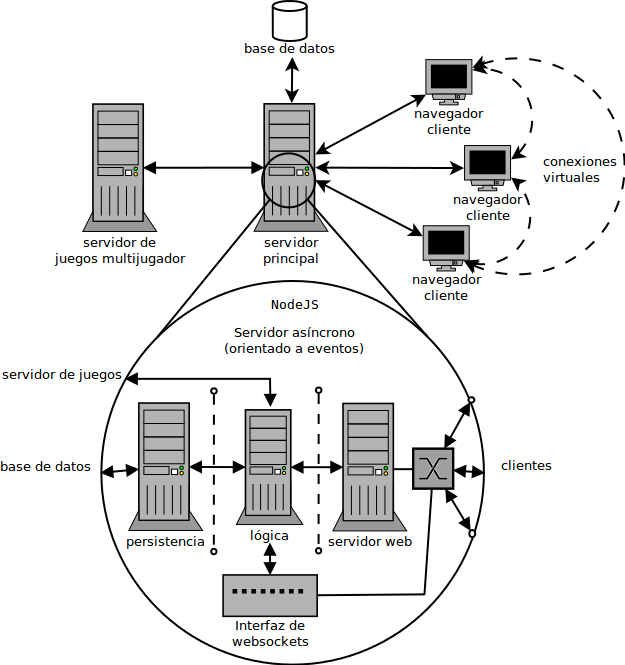
\includegraphics[width=\textwidth]{img/arquitectura.png}
    \caption{Visión global del sistema}
    \label{arquitectura}
  \end{center}
\end{figure}

\addcontentsline{toc}{section}{Referencias}
\begin{thebibliography}{100}

\bibitem{neurofisiologia}
  Georges Morin,
  \emph{Fisiología del Sistema Nevioso Central}.
  Ediciones Toray-Masson S.A.

\bibitem{fisiologia}
  Arthur C. Guyton,
  \emph{Tratado de Fisiología Médica}.
  Editora Importécnica S.A.

\bibitem{neuroplasticity}
  M.Ed. Dominick M. Maino, O.D. 
  \emph{Neuroplasticity: Teaching an old brain new tricks.}
  Jobson Publishing L.L.C., 2008.

\bibitem{matters}
  Floris de Lange.
  \emph{Matters of the brain.}
  The CFIDS Chronicle, 2006.

\bibitem{musicians}
  Thomas F. Münte, Eckart Altenmüller, and Lutz Jäncke.
  \emph{The musician’s brain as a model of neuroplasticity.}
  Nature Reviews: Neuroscience, 2002.

\bibitem{cortex}
  Dan Hackley.
  \emph{Coach your cortex}
  The Psychologist, 2011.

%%

\bibitem{goodparts}
  Doublas Crockford,
  \emph{JavaScript. The good parts}. O'Reilly

\bibitem{performance}
  Nicholas C. Zackas,
  \emph{High performance JavaScript}. O'Reilly

\bibitem{meyer}
  Eric A. Meyer,
  \emph{CSS: The definitive guide}. O'Reilly

\bibitem{jeffrey}
  Jeffrey Way,
  \emph{Decoding HTML5}. Rockable

\bibitem{byexample}
  Makzan
  \emph{HTML5. Games Development by Example}. Packt Publishing

\bibitem{canvas}
  Rob Hawkes
  \emph{HTML5 Canvas for Games and Entertainment}. Apress


\bibitem{professional}
  Nicholas C. Zackas,
  \emph{Professional JavaScript for web developers}. Wrox

\bibitem{ninja}
  John Resig et al.,
  \emph{Secrets of the JavaScript ninja}. Manning

\bibitem{pro}
  Peter Lubbers et al.,
  \emph{Pro HTML5 Programming}. Apress

\bibitem{larry}
  Larry Ullman,
  \emph{Modern JavaScript: Develop and Design}. Peachpit Press

\bibitem{maintainable}
  Nicholas C. Zackas,
  \emph{Maintainable JavaScript}. O'Reilly

\bibitem{action}
  Bear Bibeault,
  \emph{JQuery in action}. Manning


% \bibitem{google}
%   James Whittaker et al.,
%   \emph{How Google Tests Software}. Addison-Whesley

% \bibitem{testdriven}
%   Christian Johansen,
%   \emph{Test-Driven JavaScript Development}. Addison-Wesley

\bibitem{mclaughlin}
  Brett McLaughlin,
  \emph{What is Node?}. O'Reilly

\bibitem{jquery}
  JQuery,
  \emph{Official API Documentation}.\\\href{http://jquery.com/}{\tt http://jquery.com/}

\bibitem{jqueryui}
  JQuery UI,
  \emph{Official API Documentation}.\\\href{http://jqueryui.com/}{\tt http://jqueryui.com/}

\bibitem{node}
  NodeJS,
  \emph{Official API Documentation}. \href{http://nodejs.org/api/}{\tt http://nodejs.org/api/}

\bibitem{asynchronous}
  Marc Fasel,
  \emph{Asynchronous Code Design with NodeJS}.\\\href{http://goo.gl/GjcR1}{\tt http://goo.gl/GjcR1}

\bibitem{nodester}
  Nodester,
  \emph{Free open source hosting for NodeJS apps}.\\\href{http://nodester.com/}{\tt http://nodester.com/}

\bibitem{nodemanual}
  Nodemanual.org,
  \emph{NodeJS API Reference, NodeJS Guide and JavaScript Reference}. \href{http://nodemanual.org/latest/}{\tt http://nodemanual.org/latest/}

\bibitem{socketio}
  Socket.IO,
  \emph{Official Website and documentation}. \href{http://socket.io/}{\tt http://socket.io/}

\bibitem{mongodb}
  MongoDB,
  \emph{Official Website and documentation}.\\\href{http://www.mongodb.org/}{\tt http://www.mongodb.org/}

\bibitem{mongolab}
  Mongolab,
  \emph{Free open source hosting for MongoDB}.\\\href{https://mongolab.com/home}{\tt https://mongolab.com/home}

\bibitem{mongonative}
  Christian Amor Kvalheim,
  \emph{Native MongoDB connector for NodeJS}. \href{https://github.com/mongodb/node-mongodb-native}{\tt https://github.com/mongodb/node-mongodb-native}

\bibitem{json}
  JSON,
  \emph{Official website}. \href{http://www.json.org/}{\tt http://www.json.org/}

\bibitem{cocinaconmigo}
  Nintendo,
  \emph{Cocina conmigo}.
  Nintendo. \href{http://goo.gl/P2qdu}{\tt http://goo.gl/P2qdu}

\bibitem{mascotas}
  Nintendo,
  \emph{Nintendogs+Cats}.
  Nintendo. \href{http://goo.gl/eJiMb}{\tt http://goo.gl/eJiMb}

\bibitem{braintraining}
  Dr. Kawashima,
  \emph{Brain Training}.
  Nintendo. \href{http://goo.gl/EXzIn}{\tt http://goo.gl/EXzIn}

\bibitem{brainarena}
  Brainarena,
  \emph{Web oficial}. \href{http://brainarena.com/}{\tt http://brainarena.com/}

\bibitem{lumosity}
  Lumosity,
  \emph{Improve your brain health and performance}. \href{http://www.lumosity.com}{\tt http://www.lumosity.com}


\end{thebibliography}


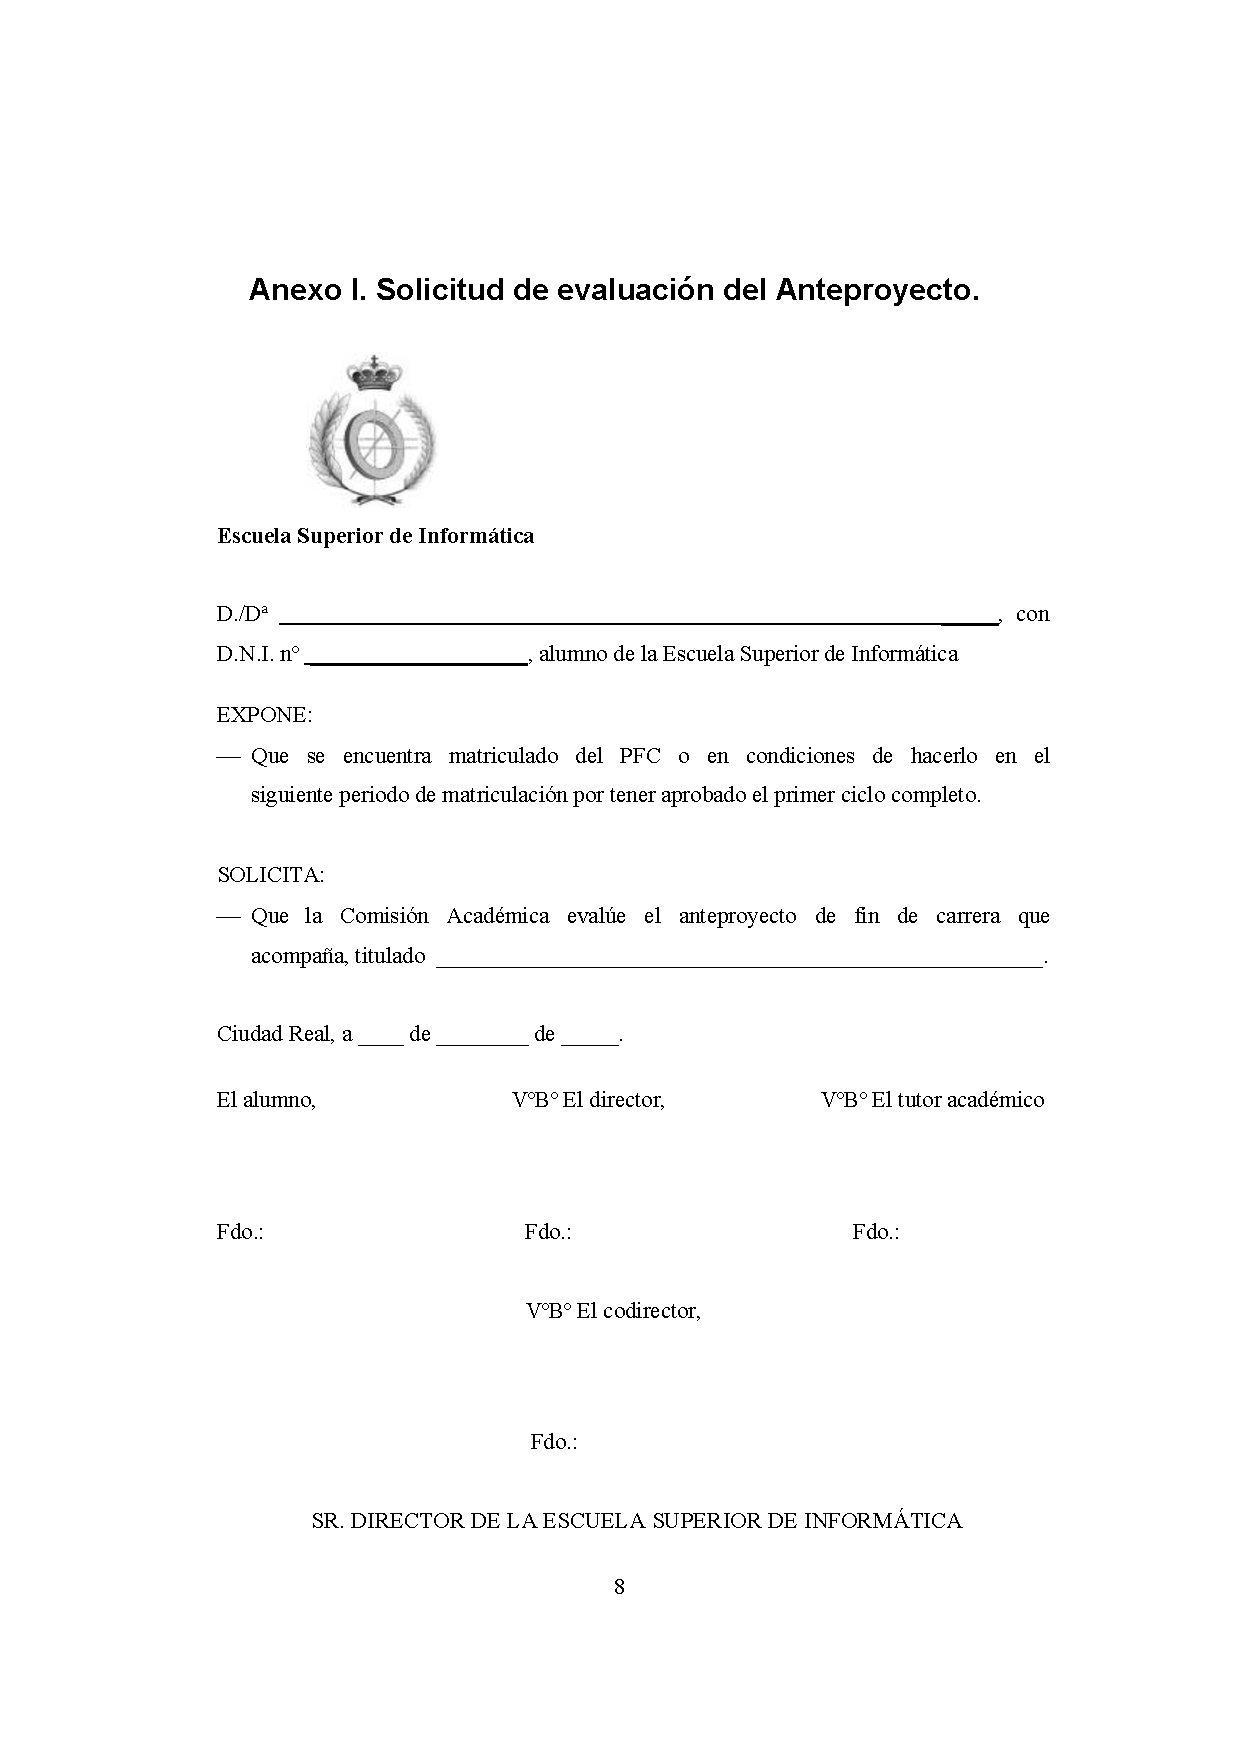
\includepdf[pages={1}]{anexo1.pdf}

%%%%%%%%%%%%%%%%%%%%%%%%%%%%%%%%%%%%%%%%%%%%%%%%%%%%%%%%%%%%%%%%%%%%%%%%%%%%%%%%
%% HASTA AQUÍ %%%%%%%%%%%%%%%%%%%%%%%%%%%%%%%%%%%%%%%%%%%%%%%%%%%%%%%%%%%%%%%%%%
%%%%%%%%%%%%%%%%%%%%%%%%%%%%%%%%%%%%%%%%%%%%%%%%%%%%%%%%%%%%%%%%%%%%%%%%%%%%%%%%

\end{document}
